\documentclass{beamer}
\usepackage{subfig}
\usepackage{amsmath}
\usepackage{bm}

\DeclareMathOperator*{\argmax}{arg\,max}
\DeclareMathOperator*{\argmin}{arg\,min}


\title{Neural Networks}
\author{Prof. Alessandro Lucantonio}
\institute{Aarhus University}
\date{7/11/2023}

\setbeamertemplate{footline}[frame number]
\setbeamertemplate{navigation symbols}{}


\begin{document}
	\frame{\titlepage}
	
	\begin{frame}
		\frametitle{Introduction}
		\begin{itemize}
			\setlength\itemsep{5mm}
			\item Neural Networks (NN) are one of the most flexible ML tools
			\item \textit{Universal approximators}
			\item Can manipulate continous and discrete data $\leadsto$ regression and classification problems
			\item Not a single model: many types of NN (e.g. MLP, CNN, RNN)
			\item (Loosely) inspired by biological systems
		\end{itemize}
	\end{frame}

	\begin{frame}
	\frametitle{Perceptron}
	\begin{figure}
		\centering
		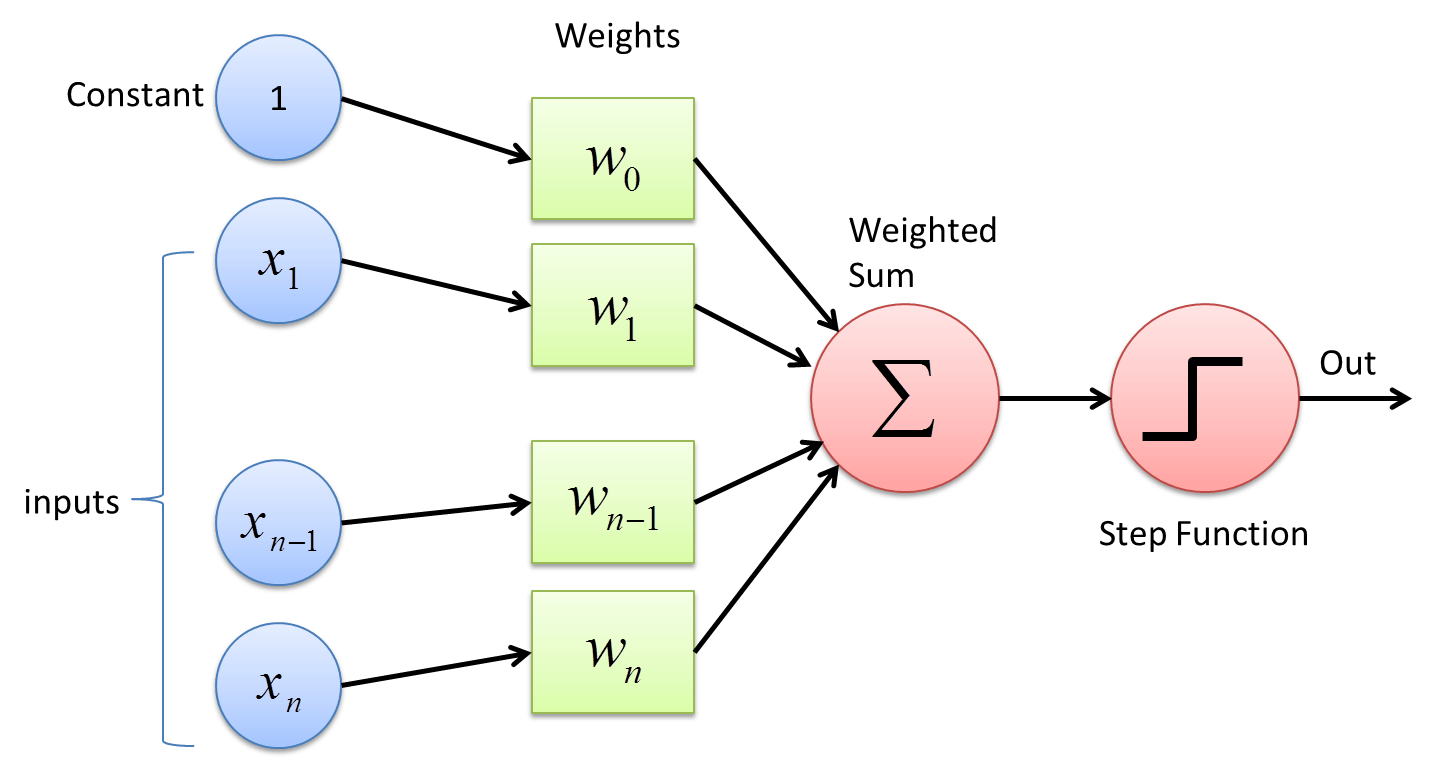
\includegraphics[scale=0.2]{images/perceptron}
		\caption{Representation of a perceptron.}
	\end{figure}
\end{frame}


	\begin{frame}
		\frametitle{Multi-Layer Perceptron (MLP)}
		The MLP is a fundamental type of NN: it consists of three types (input, hidden, output) of fully-connected layers such that information flows forward from the inputs to the output.
		\begin{figure}
			\centering
			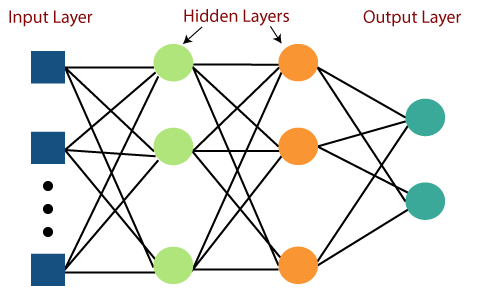
\includegraphics[scale=0.35]{images/mlp-visualization}
		\end{figure}
	\end{frame}



%	\begin{frame}
%		\frametitle{Introduction - Convolutional Neural Networks (CNN)}
%		CNN are the foundations of Deep Learning. Its name derive from the fact that they use a special operation, called \textsl{convolution}.
%		\begin{figure}
%			\centering
%			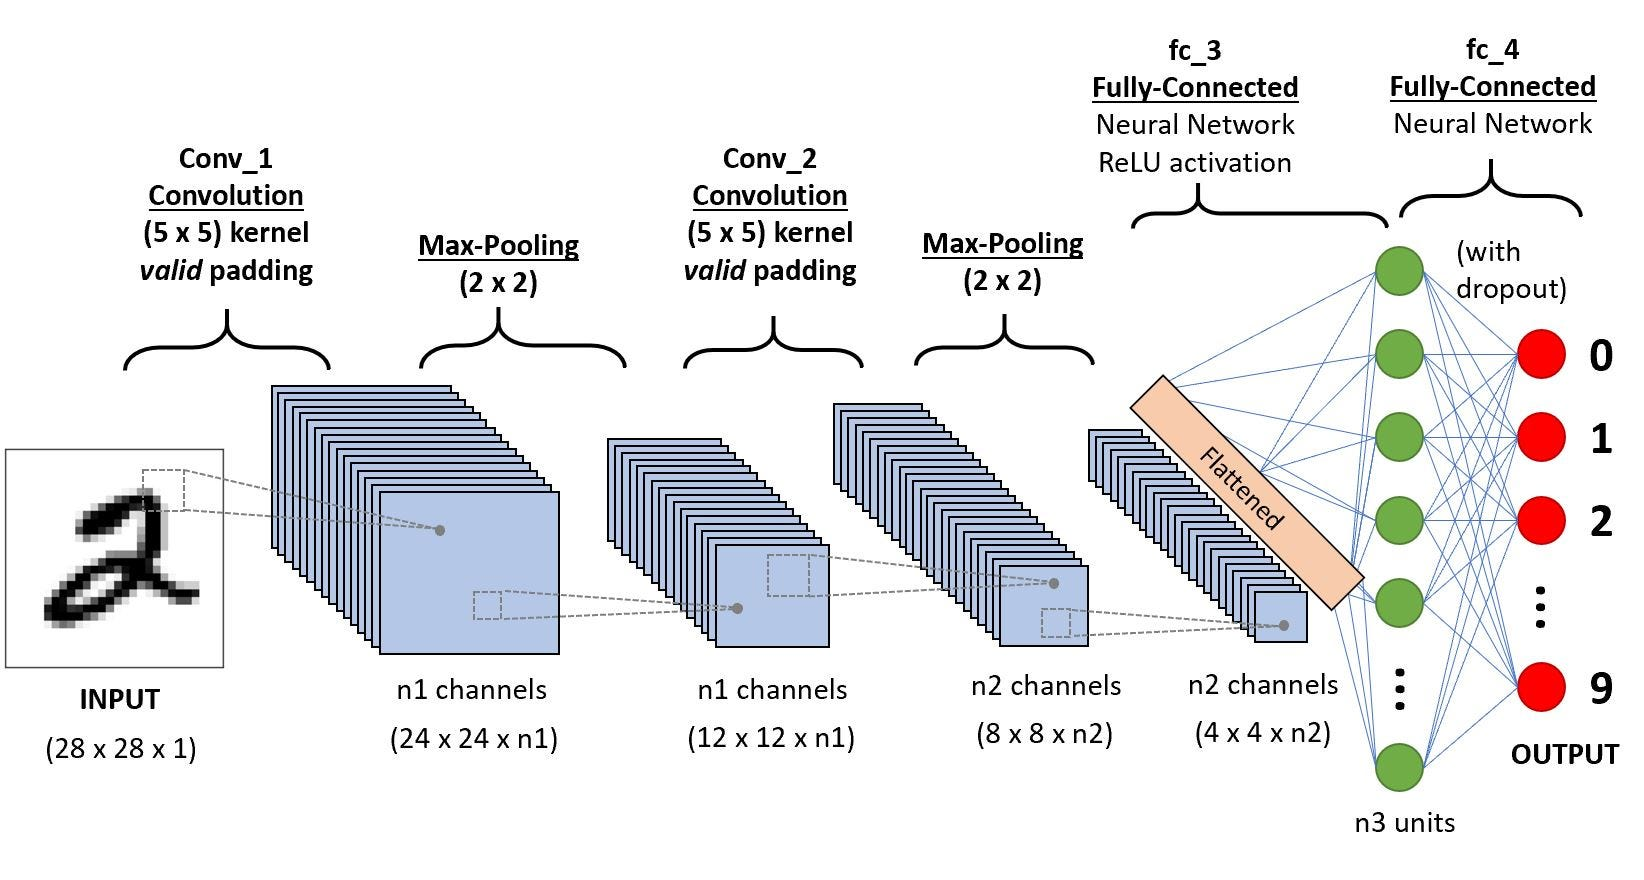
\includegraphics[scale=0.15]{images/cnn}
%		\end{figure}
%	\end{frame}

%	\begin{frame}
%		\frametitle{Introduction - Recurrent Neural Networks (RNN)}
%		RNN constitute a class of NN where connections between nodes can create a cycle. In particular, they admit output from some nodes to affect subsequent input to the same nodes.
%		\begin{figure}
%			\centering
%			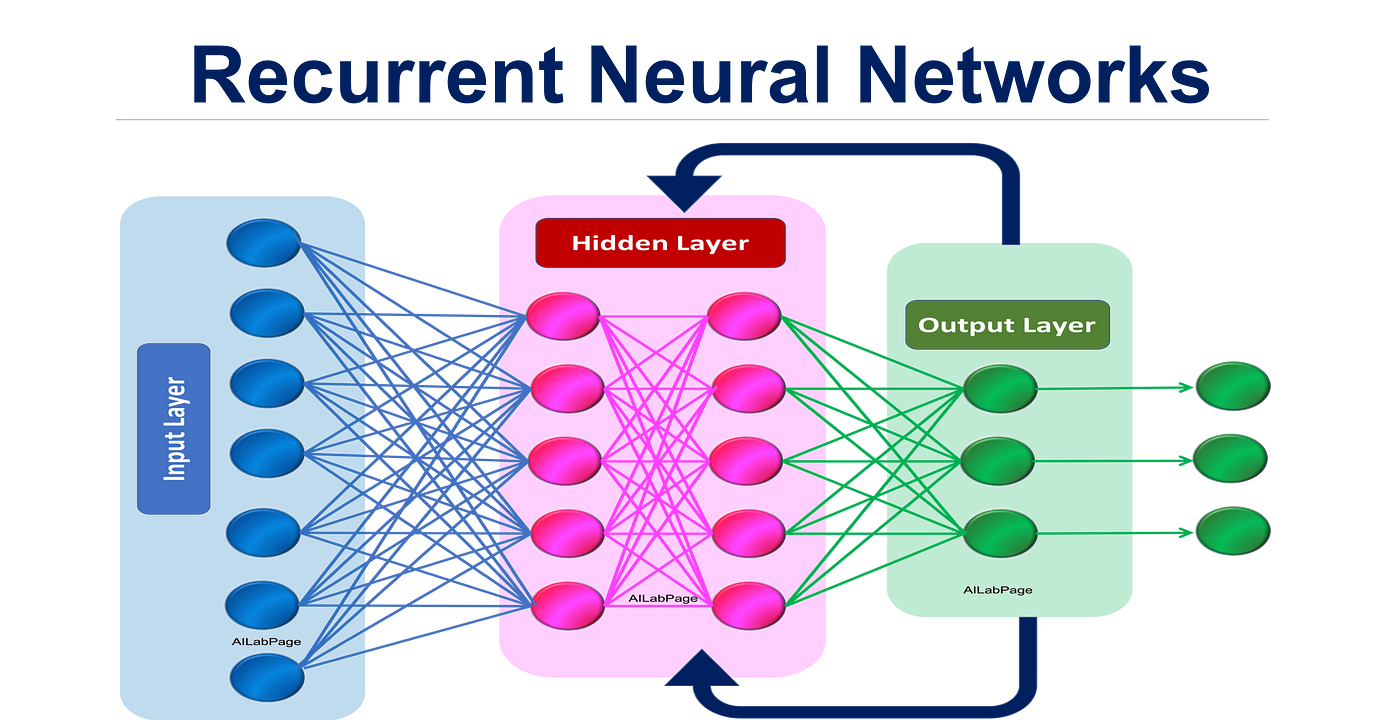
\includegraphics[scale=0.20]{images/rnn}
%		\end{figure}
%	\end{frame}
	

	\begin{frame}
		\frametitle{Perceptron - Formal}

		Operation of a single unit:
		\begin{equation*}
			\begin{cases}
				z(\bm{x}) := \bm{w}^T \bm{x} + \bm{b}\\
				h(\bm{x}) := f(z(\bm{x}))
			\end{cases}
		\end{equation*}
	
		with $z$  the \textbf{net input} to the neuron, $ \bm{b}$ is the \textbf{bias} and $f$ is the \textbf{activation function}. 
		
		\vspace{5mm}
		
		Examples of activation functions:
		\begin{itemize}
			\item Linear:  $f(t) = at + b$
			\item ReLU (Rectified Linear Unit): $f(t) := \max\{0, t\}$
			\item Sigmoid: $f(t) := \frac{1}{1 + e^{-t}}$
			\item Tanh (Hyperbolic tangent): $f(t) := \frac{e^{2t}-1}{e^{2t}+1}$
		\end{itemize}
		
	\end{frame}
	
	\begin{frame}
		\frametitle{Activation functions - Plots}
		\begin{figure}
			\centering
			\subfloat[Linear]{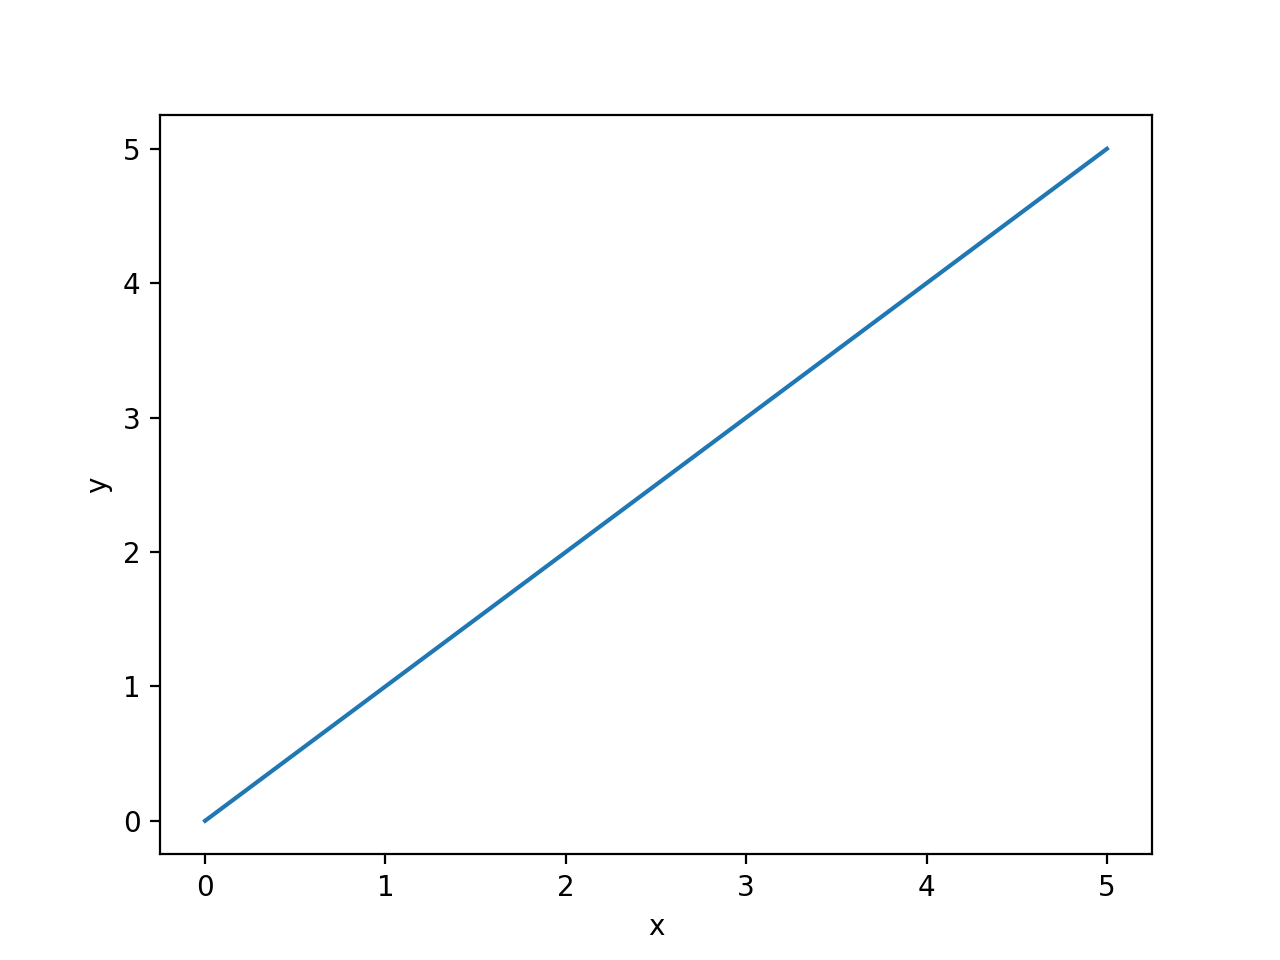
\includegraphics[scale=0.25]{images/linear}}
			\qquad
			\subfloat[ReLU]{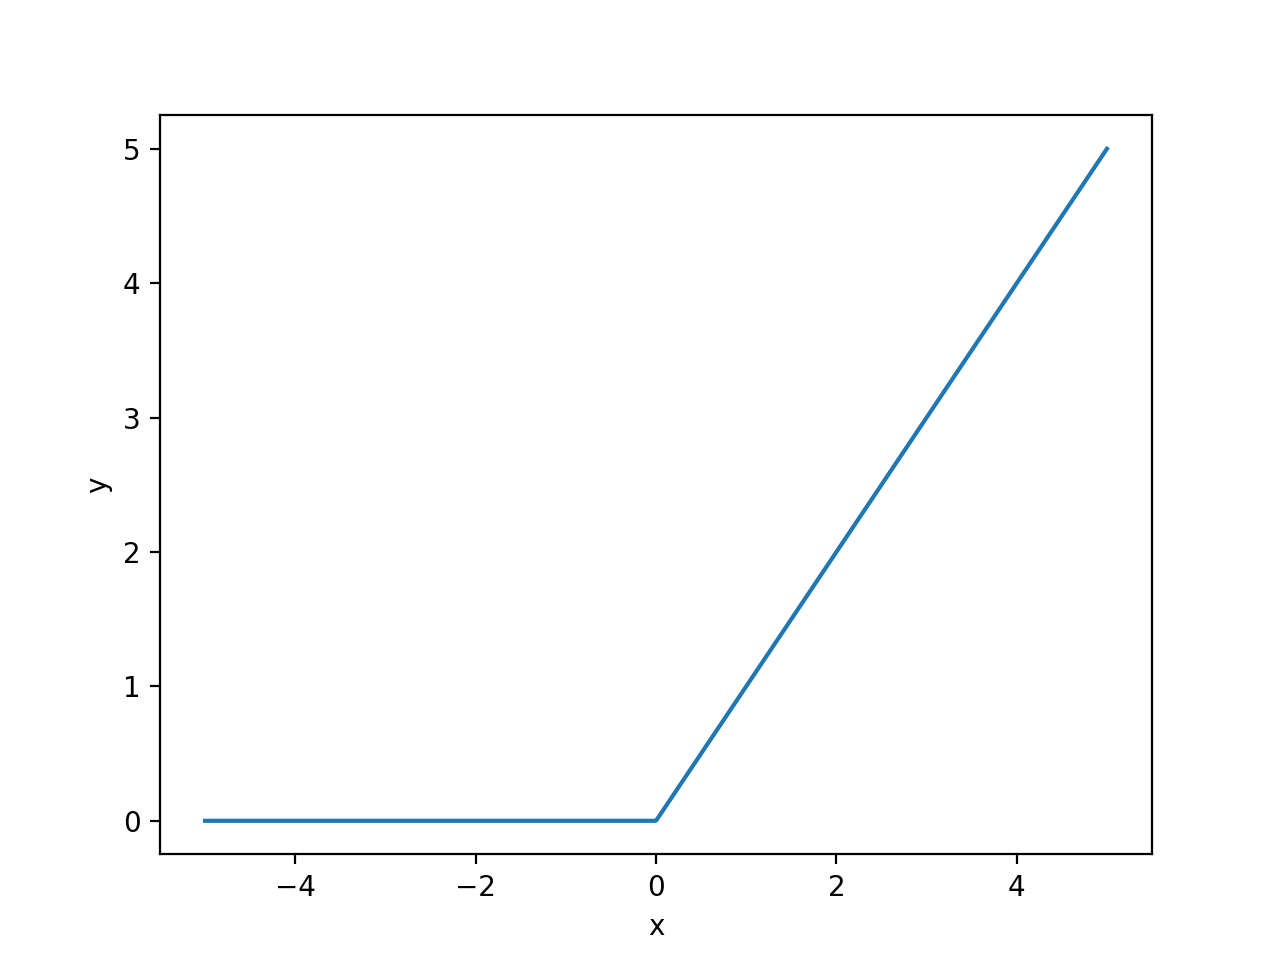
\includegraphics[scale=0.25]{images/relu}}
			\\ \vspace{0.1cm}
			\subfloat[Sigmoid]{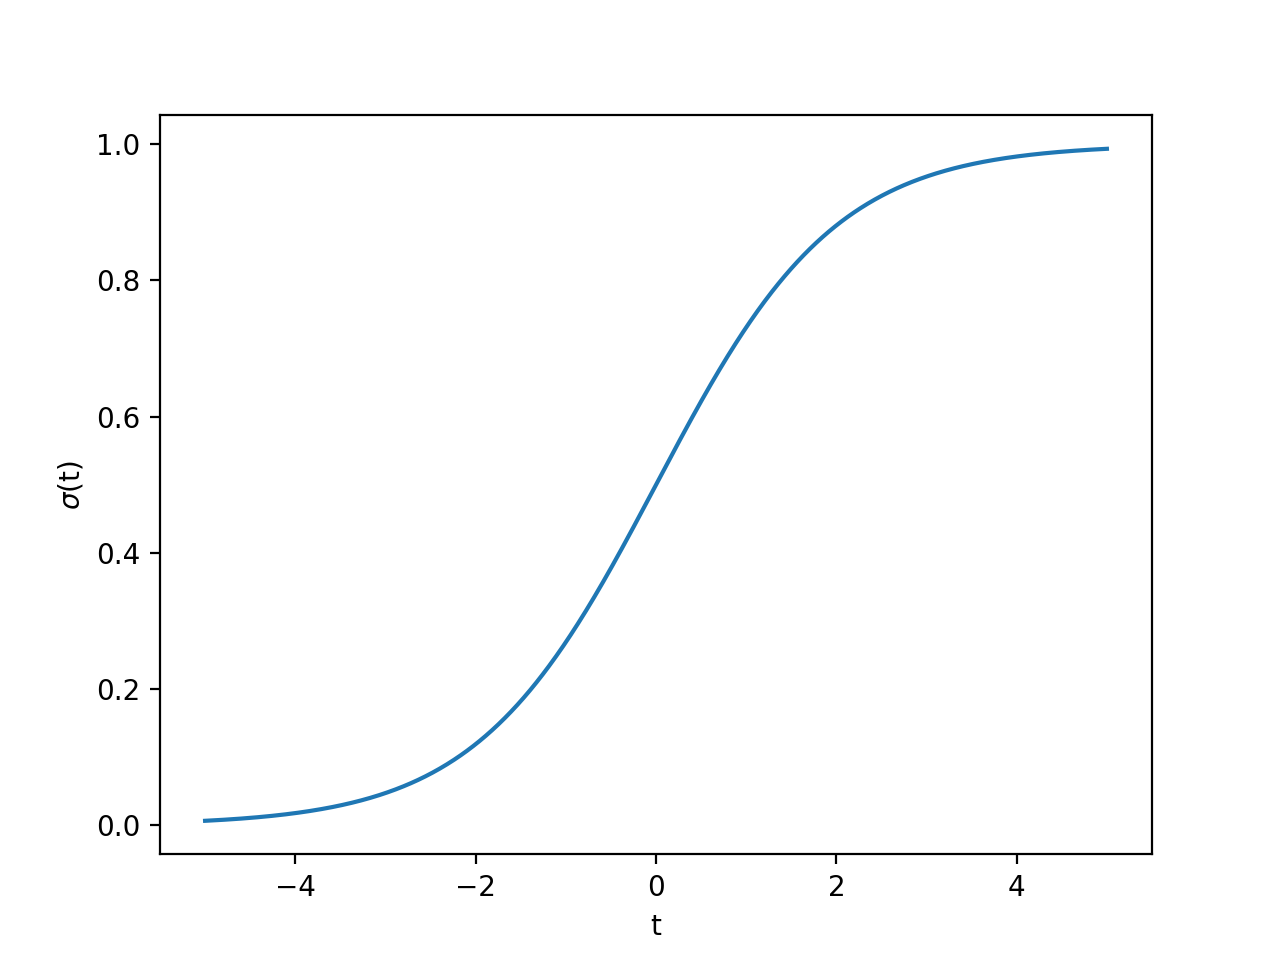
\includegraphics[scale=0.25]{images/sigmoid}}
			\qquad
			\subfloat[Tanh]{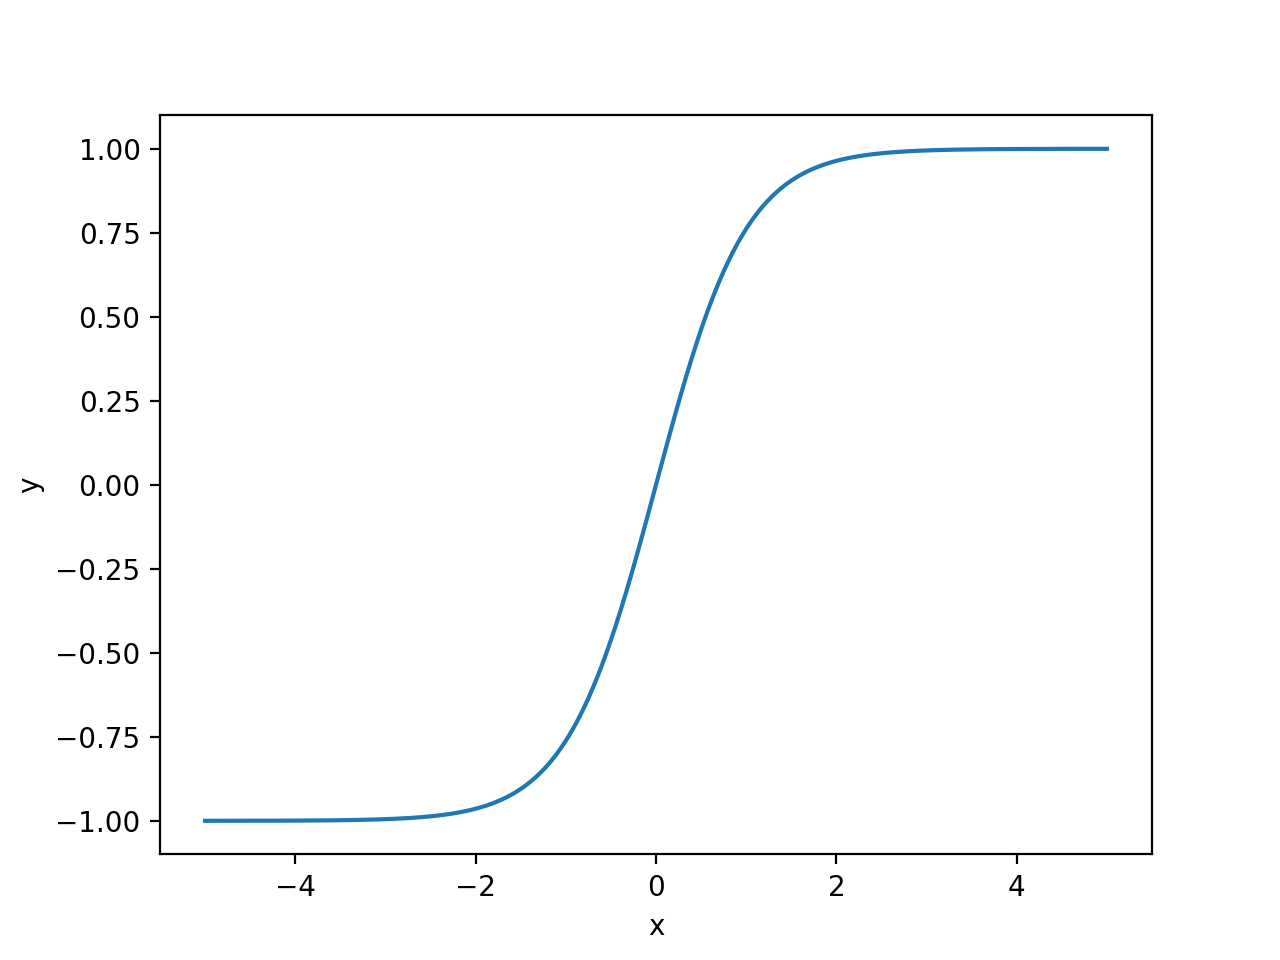
\includegraphics[scale=0.25]{images/tanh}}
		\end{figure}
	\end{frame}
	
	\begin{frame}
		\frametitle{Activation functions - Features}
		\begin{itemize}
			\item ReLU: excellent default choice (easy to optimize because they are similar to linear units), the derivative remains large when active,  disregard the non-differentiability
			\item Sigmoid: saturates when the argument is either very positive or very negative $\leadsto$ gradient-based learning may be hard, better not to use them as hidden units unless appropriate cost function can undo the saturation in the output layer (when output is a probability)
			\item Tanh: performs better than sigmoid when the latter must be used, similar to the identity near 0, composition of two tanh resembles a linear model as long as the argument is small (easier training)
		\end{itemize}
	\end{frame}

	\begin{frame}
		\frametitle{MLP representation - Formal}
		Notation: 
		\begin{itemize}
			\item $\bm{a}^{(j)}$ is the output of the $j$-th layer
			\item $\mathsf{W}^{(j)}$ is the weight matrix for the inputs of the $j$-th layer
			\item $m$ is the number of layers (including input and output)
		\end{itemize}
				
		\vspace{5mm}
				
		For each layer $j = 1, \dots, m-1$ compute:
		\begin{equation*}
			\begin{cases}
				\bm{z}^{(j)}(\bm{a}^{(j-1)}) := \mathsf{W}^{(j)} \bm{a}^{(j-1)} + \bm{b}^{(j)},\\
				\bm{a}^{(j)} := h^{(j)}(\bm{a}^{(j-1)}) = f^{(j)}(\bm{z}^{(j)}(\bm{a}^{(j-1)})).
			\end{cases}
		\end{equation*}
		with 
		$\bm{a}^{(0)} = \bm{x}$ (notice: no 1 in the first entry) and $\bm{a}^{(m-1)}$ is the output of the network.

	\end{frame}

	\begin{frame}
		\frametitle{MLP representation - Multiple samples}
		For each layer $j = 1, \dots, m-1$ compute:
		\begin{equation*}
			\begin{cases}
				\mathsf{Z}^{(j)}(\mathsf{A}^{(j-1)}) := \mathsf{A}^{(j-1)}\mathsf{W}^{(j)}  + (\bm{b}^{(j)})^T,\\
				\mathsf{A}^{(j)} := h^{(j)}(\mathsf{A}^{(j-1)}) = f^{(j)}(\mathsf{Z}^{(j)}(\mathsf{A}^{(j-1)})).
			\end{cases}
		\end{equation*}
		with $\mathsf{A}^{(j)}$ the \textit{matrix} of the outputs of the $j$-th layer (rows correspond to samples) and $\mathsf{A}^{(0)} = \mathsf{X}$ (\textbf{without} the column of ones). Here, $(\bm{b}^{(j)})^T$ is a \textit{row vector} containing the biases (use \href{https://numpy.org/doc/stable/user/basics.broadcasting.html}{\textit{broadcasting}} to extend it to $N$ samples).
		
		\begin{figure}
			\centering
			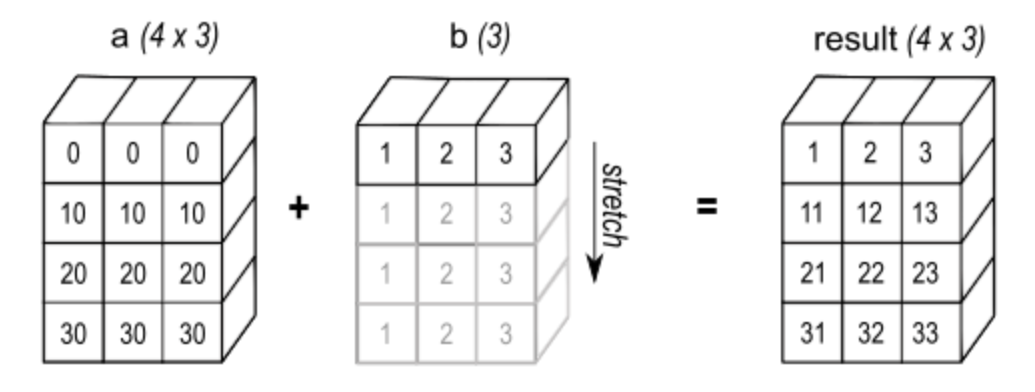
\includegraphics[scale=0.3]{images/broadcasting.png}
			\caption{Array broadcasting in NumPy.}
			\label{fig:broadcasting}
		\end{figure}
		
	\end{frame}

	\begin{frame}
		\frametitle{MLP representation - Example}
		Assume single sample, 3 inputs, 1 hidden layer/4 units, 1 output:
		\tiny{
		\begin{itemize}
			\item $\bm{x}$ is a 3x1 vector
			\item $\bm{b}^{(1)}$ is a 4x1 vector
			\item $\mathsf{W}^{(1)}$ is a 4x3 matrix (each row contains the weights relative to a unit of the hidden layer)
			\item $\bm{z}^{(1)}$ is a 4x1 vector (each component corresponding to the net input of a unit of the hidden layer)
			\item $\bm{a}^{(1)}$ is a 4x1 vector (each component corresponding to the output of a unit of the hidden layer)
			\item $\mathsf{W}^{(2)}$ is a 1x4 matrix
			\item $\bm{b}^{(2)}$ is a 1x1 vector
			\item $\bm{a}^{(2)} = \bm{z}^{(2)}$ is a 1x1 vector (output)
		\end{itemize}}
	\normalsize
		Calculations with component notation:
		$$\bm{z}_i^{(1)} = \mathsf{W}_{ik}^{(1)}\bm{x}_k + \bm{b}^{(1)}_i, \quad i=1,2,3,4$$
		$$\bm{a}_i^{(1)} = h_i^{(1)}(\bm{z}^{(1)}), \quad i=1,2,3,4 $$
		$$\bm{a}_1^{(2)} = \bm{z}_1^{(2)} = \mathsf{W}_{1k}^{(2)}\bm{a}^{(1)}_k + \bm{b}_1^{(2)}$$
	\end{frame}
	
	\begin{frame}
		\frametitle{Learning XOR with an MLP}
		Architecture: 1 hidden layer containing 2 ReLU units.
		
		\vspace{5mm}
		
		Call $\mathsf{W} = \mathsf{W}^{(1)}$, $\bm{b}^{(1)} = \bm{b}$ and $\bm{w} =  \mathsf{W}^{(2)}$. Set $\bm{b}^{(2)} = \bm{0}$.
		
		\vspace{5mm}
		
		A solution to the problem is:
		$$\mathsf{W} = \begin{bmatrix}
			 1 & 1\\
			 1 & 1
		\end{bmatrix} \quad 
		\bm{b} = \begin{bmatrix}
		0 \\
		-1
		\end{bmatrix} \quad 
		\bm{w} = \begin{bmatrix}
			1 \\
			-2
		\end{bmatrix}
		$$
		
		Indeed, for the set of inputs
		$$\mathsf{X} = \begin{bmatrix}
			0 & 0\\
			0 & 1 \\
			1 & 0 \\
			1 & 1
			\end{bmatrix}
		$$
		the output $\bm{w}^T \max \{0, \mathsf{XW} + \bm{b}^T\}$ is $[0, 1, 1, 0]^T$.
		
		\vspace{5mm}
		
		\textbf{Exercise}: try to solve the problem using \textit{Linear Regression}.
		
	\end{frame}

	\begin{frame}
	\frametitle{MLP - Features}
	\begin{itemize}
		\setlength\itemsep{5mm}
		\item This type of NN is also called \textbf{feedforward NN} because information flows from input to output without feedback
		\item The hypothesis function is \textit{ non-convex} because composition of convex functions is not necessarily convex
		\item Theory tells us that one-layer MLPs are \textbf{universal approximators}, \textit{i.e.} they approximate \textit{any continuous function} with any desired accuracy (not a formal statement), even though the layer may be infeasible large and may fail to learn and generalize correctly
	\end{itemize}
\end{frame}

	\begin{frame}
		\frametitle{Tips and Tricks - Is one layer really enough?}
		Theory suggests us that the answer is yes, but pay attention: \textit{an exponential number of hidden units} (w.r.t. the input dimension) may be needed to approximate well the data, \textit{i.e.} one hidden unit for each input configuration that needs to be distinguished.
		
		\vspace{5mm}
		\begin{itemize}
			\item Empirically, increasing the \textit{depth} results in better generalization for a wide variety of tasks (even though training is harder)
			\item Try different architectures in the model selection
		\end{itemize}
		
	\end{frame}

	\begin{frame}
		\frametitle{Back-propagation}
		For network training via gradient descent, we need to compute the gradient of the cost with respect to the weights and biases.
		
		We use \textbf{back-propagation}, which allows the information from the cost to then flow backward through the network.
		
		\begin{itemize}
			\item NNs are represented as \textbf{computational graphs}
			\item the \textit{chain rule of Calculus} is used to compute derivatives by composing operations in a specific order that is highly efficient
		\end{itemize}
		
		\begin{figure}
			\centering
			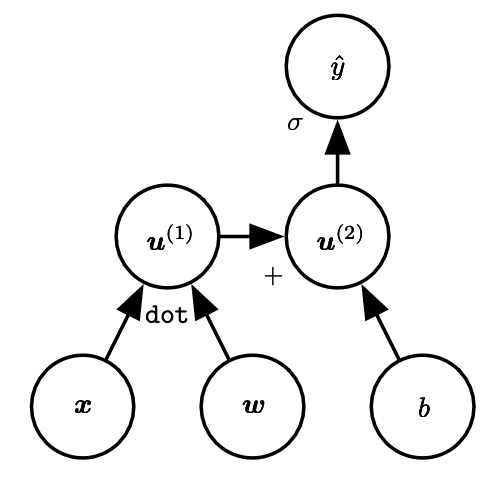
\includegraphics[scale=0.35]{images/graph1}
			\caption{Example of computational graph of the function $\hat{y} = \sigma(\bm{w}^T\bm{x}+b)$.}
		\end{figure}
	\end{frame}

	\begin{frame}
		\frametitle{Back-propagation - Example}
		\tiny
		\begin{itemize}
			\item \textit{Forward pass}: Compute the output $E$ given the inputs $\bm{x}$ following the operations of the graph.
			\begin{align*}
				&u^{(1)} = \bm{w}^T\bm{x} \\
				&u^{(2)} = u^{(1)} + b \\
				&\hat{y} = \sigma(u^{(2)}) \\
				&E = \textrm{MSE}(\hat{y}-y) = (\hat{y}-y)^2
			\end{align*}
			\item \textit{Backprop}:
			For each operation (node) in the graph starting from the output and going backward, compute the gradient of the output $E$ with respect to the inputs of that operation and propagate this information to the \textit{parents} of the graph node to eventually compute the derivatives of $E$ with respect to weights $\bm{w}$ and bias $b$.
			\begin{align*}
				&\frac{\partial E}{\partial \hat{y}} = 2(\hat{y}-y) \\
				&\frac{\partial E}{\partial u^{(2)}} = \frac{\partial E}{\partial \hat{y}} \frac{\partial \hat{y}}{\partial u^{(2)}} = 2(\hat{y}-y) \sigma'(u^{(2)})\\
				&\frac{\partial E}{\partial u^{(1)}} = \frac{\partial E}{\partial u^{(2)}}  \frac{\partial u^{(2)}}{\partial u^{(1)}}  = 2(\hat{y}-y) \sigma'(u^{(2)})  \\
				&\frac{\partial E}{\partial b}  = \frac{\partial E}{\partial u^{(2)}}  \frac{\partial u^{(2)}}{\partial b}  = 2(\hat{y}-y) \sigma'(u^{(2)})\\
				&\frac{\partial E}{\partial \bm{w}}  =\frac{\partial E}{\partial u^{(1)}} \frac{\partial u^{(1)}}{\partial \bm{w}}= 2( \sigma( \bm{w}^T\bm{x} +b)-y) \sigma'( \bm{w}^T\bm{x} +b) \bm{x}
			\end{align*}
		\end{itemize}
		
	\end{frame}

	\begin{frame}
		\frametitle{Tips and Tricks - NN best practices}
		\begin{itemize}
			\item Initialize all weights \textit{randomly} near zero (or use other initialization techniques), but \textbf{do not} initialize uniformly to \textit{break symmetry} and avoid \textit{vanishing/exploding gradients}
			\item If a learning algorithm is suffering from \textit{high bias}, getting more training data will not (by itself) help much. Instead, if a learning algorithm is suffering from \textit{high variance}, getting more training data is likely to help
			\item Fewer features fixes \textit{high variance} but not high bias; additional features fixes \textit{high bias} but not high variance
			\item In general, use regularization to counter overfitting
			\item Small (big) NNs are more prone to underfitting (overfitting); use cross-validation to select network size
		\end{itemize}
	\end{frame}
	
	\begin{frame}
		\frametitle{Basic Recipe for Machine Learning}
		\begin{itemize}
			\item If your model has a high bias:
			\begin{itemize}
				\item Try to make your NN bigger (number of hidden units, number of layers)
				\item Try a different model that is suitable for your data
				\item Try to increase the number of epochs
			\end{itemize}
			\item If your model has a high variance:
			\begin{itemize}
				\item More data
				\item Try regularization
				\item Try a different model that is suitable for your data
			\end{itemize}
			You should try the previous two points until you achieve low bias and low variance.
		\end{itemize}
	\end{frame}
\end{document}

% NEXT LECTURE:
% learning rate decay, early stopping, dropout, ensemble, Adam/momentum, batch normalization